
\tableofcontents

\verbatimfont{\footnotesize}%

\newcommand{\TODO}[1]{\todo[inline]{#1}}

\begin{abstract}

Today's tasks require a plethora of analytics tasks to be conducted to
tackle state-of-the-art computational challenges posed in society
impacting many areas including health care, automotive, banking,
natural language processing, image detection many more data analytics
related tasks. Leveraging existing analytics functions from each other allows reuse and reduces overall effort. However, integrating such frameworks in the age of cloud computing is often out of reach for the domain experts. Simple frameworks are needed that allow even non experts to deploy and host services in the cloud. To avoid vendor lock-in, we require a generalized composable analytics service framework that allows users to integrate their own services and those offered in clouds, not only one but by many cloud compute and service providers.

We report on work that we conducted to  provide a service integration framework for compose generalized analytics frameworks on multi cloud providers. We demonstrate the usability of the framework by showcasing useful analytics workflows on various cloud providers including AWS, Azure, and Google and edge computing IoT devices. The examples, are based on Scikit learn in order to use them also in educational settings that can be easily replicated and expanded upon. Benchmarks are used to compare the different services and showcase general replicatibility.


\end{abstract}

\maketitle

\textbf{Keywords:} cloudmesh, AI service, REST, multi-cloud

\section{Introduction}


In today's application scientist want to share their services with a wide number of colleagues while not only offering the services as bare metal programs, but exposing the functionality as a software as a service. This has the advantage that the services can be readily be reused in other applications and hosted on the cloud allowing access to state-of-the art or volumes of resources that otherwise would not be accessible to individual domain experts. Through the increased availability resource constraints can be reduced and scientists can offer their analytics workflows as services to the community. This may include long lasting services envisioned by cloud computing as part of its Software as a Service (SaaS) paradigm or for smaller analytics functions as microservices. Furthermore, a subset of analytics functions can be offered as part of serverless computing elevating the penetration from a pure bare metal solution to a multi-pronged cloud based service offering.

While working with a number of professionals, researchers, and students we found that the entry level to accomplish this goal is very high and it will elude many of the domain experts as they neither have the expertise nor do they have the time to learn the expertise necessary to conduct the infrastructure related tasks integrating DevOps and analytics tasks. Although recent developments especially on the serverless computing side have made progress, we ought to be able to leverage the existing expertise of the domain scientists while automating the creation of various services from SaaS, microservices and serverless computing.
Having worked with this community we found that the educational steps involved for a beginner take about 2 to three month to get up to a level where development of cloud based services is possible. We set the goal to explore if it is possible to reduce drastically the time needed to create such services.

For this reason we developed a sophisticated but easy to use framework that takes a regular python function and converts it automatically into a secure REST service and OpenAPI specifications \cite{openapi} that can be reused in the ecosystem of cloud services. We used this framework to create a number of AI-based REST services to showcase validity of the approach. We used examples from SciKit Learn \cite{scikit-learn} and benchmark the execution of the resulting REST services on various clouds as well as on an IoT device. 

\TODO{Paper structure}

The paper is structured as follows. In Section \ref{sec:background} we will start with a very brief background section as to allow domain experts to catch up with the terminology and concepts used in our architecture. The background analysis leads us to our requirements presented in Section \ref{sec:requirements} and our architectural design shown in Section \ref{sec:architecture}. Our benchmarks are collected in Section \ref{sec:benchmark}. We present our conclusion in Section \ref{sec:conclusion}.

In the appendix a small number of useful notes are provided so ease replication of what we have achieved by others. In the final publication the appendix can be removed with a link to our manual for the pilot framework presented here \cite{cloudmesh-manual, cloudmesh-openapi} where we will include the content of the appendix. 

\section{Background}
\label{sec:background}

We provide in this background section a small summary of activities related to this research so that domain experts can get a small introduction on concepts that we use as part of the implementation of our architecture. It is beyond the scope of this paper to give a more detailed introductions in topics such as IaaS, SaaS, microserices, serverless computing, OpenAPI, and REST services. The sections will however be useful as a starting point for further research to the reader. 

\subsection{The Big Data Reference Architecture}

NIST has developed a Big Data Reference Architecture as part of
NBDIF\cite{nist-v6} and identified a number of use cases that motivate
it \cite{nist-v3}. The reference architecture is depicted in Figure \ref{fig:bdra}. It includes the following components: Data Provider, Big Data Application Provider, Big Data Framework Provider, Data Consumer and
System Orchestrator as well as two overarching fabrics: Security and
privacy and system Management. There are three types of linkages,
namely \emph{Big Data Information flow}, \emph{Service Use and
  Software Tools}, and \emph{algorithms transfer}. The architecture
presents a level of abstraction to define Big Data
applications. Components that implement sophisticated functionality
work in concert to address the challenging creation of instantiating
of architectures beyond the conceptual stage. As such, the components
interact with each other that are expressed through the linkages
within the NBDIF.  The next logical step is to explore how it can
benefit and be used for analytics services.

\begin{figure}[htb]
\centering

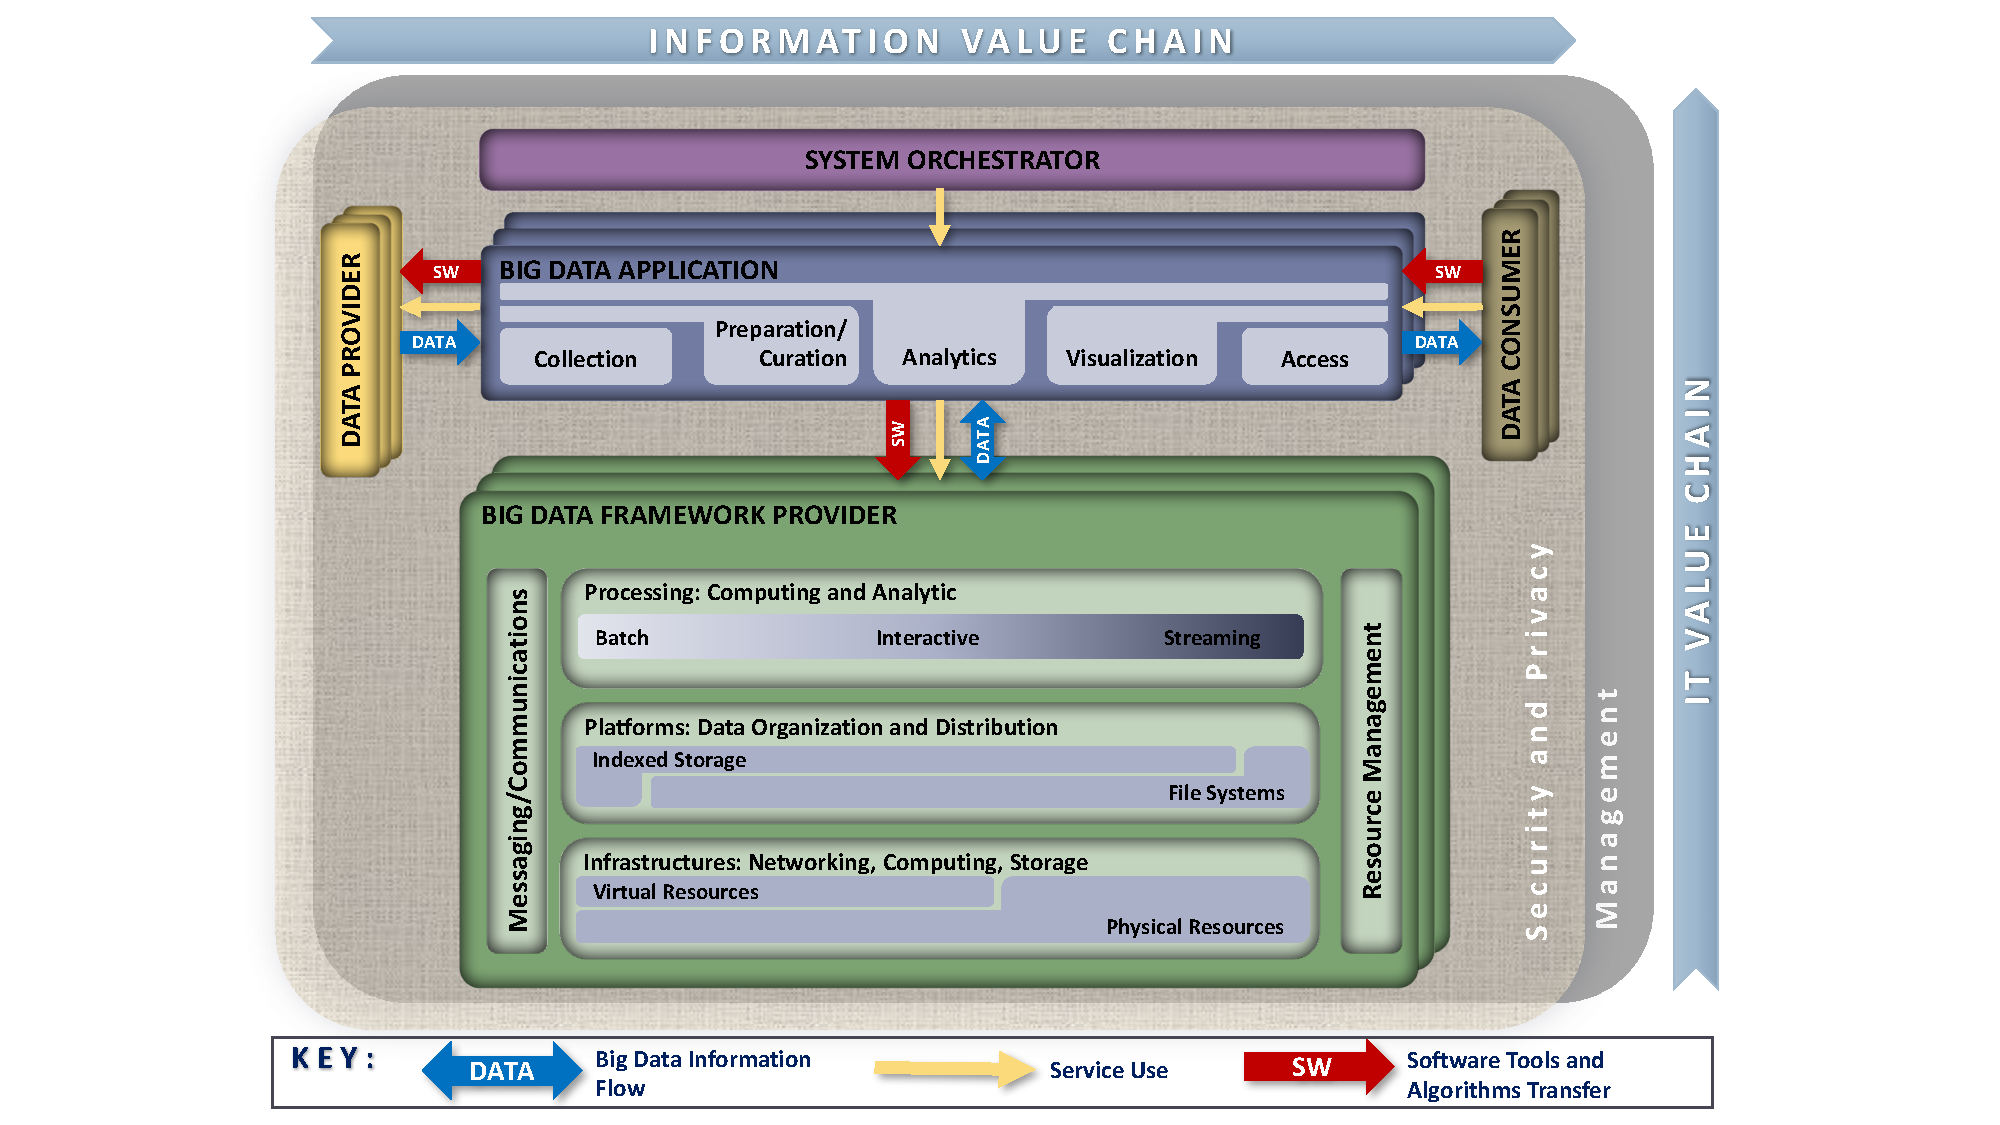
\includegraphics[width=1.0\columnwidth]{images/NIST_RA_latest.pdf}

\caption{NIST Big Data Reference Architecture \cite{nist-v8}}

\label{fig:bdra}
\end{figure}

NIST has developed through open working group participation the
following documents related to the
NBDIF~\cite{nist-v1,nist-v2,nist-v3,nist-v4,nist-v5,nist-v6,nist-v7,nist-v8,nist-v9}. Within
these activities, Volume 8 is of especial importance as it allows a
vendor-neutral specification of cloud services targeting a selected
set of Big Data Architectural needs
\cite{cloudmesh-rest,cloudmesh-book}. This effort builds the basis of
our activities reported here while expanding it to cloud providers and
services focusing on {\em Analytics Services}, which are not covered
by the current volumes. 

In a previous effort we have developed a reference implementation that follows the architecture layed out in NBDIF and is easy to use by by scientists. 
However, it focused mostly on a multi-cloud provider access via REST services and command line tools. The reference implementation is done as part of the cloudmesh project which was one of the first multi-cloud provider interfaces even including cloud technologies that are no longer active such as Eucalyptus \cite{??}, OpenCirrus \cite{??}, FutureGrid \cite{??}, and Comet Cloud \cite{??}. Today, it supports clouds such as AWS \cite{www-aws}, Azure \cite{www-azure}, Google Cloud Platform \cite{??}, Oracle \cite{??}, and OpenStack \cite{www-openStack}. It will offer value adds as it also explores the integration of MapReduce frameworks such as Hadoop \cite{??} and Spark \cite{??}, as well as container based frameworks such as Docker \cite{??} and Kubernetes \cite{??}. 

However, the work presented here focuses on the creation of analytics services that can be automatically created and hosted on any of the clouds supported by cloudmesh. This is a non trivial effort due to the large number of technologies involved and is outside of the expertise of domain scientists. However, the use of cloudmesh makes it possible that domain scientist can much more easily access these services and leverage our more than 10 years of experience in this field.

The previous work provides us with a blueprint on how to proceed.  We list the following main findings of our earlier work that we leverage as part of this work.

\begin{description}
  
\item[Software Defined Analytics Services and Applications.] Just as
  in the NBDIF the utilization of \emph{DevOps} to deliver
  Software-Defined (SD) Big Data applications is of
 utmost importance for the design of reusable services and components \cite{cloudmesh-manual,bigdata-stack-1,bigdata-stack-2}. 
  
\item[Multi-cloud Provider Interfaces.] Volume 8 was through community
  input shaped in such a form that it allows multi-cloud
  interfaces. Such interfaces have been in practical use in our
  software and showcase the validity of NIST-BDRA approach. It is
  clear that we need to to introduce such multi-cloud and multi-service
  interfaces also for analytics-related tasks whenever possible as motivated in our introduction. 

\item[Use Case Collection.] NIST has provided as part of the NIST BDRA
  document Vol. 6~\cite{nist-v6} a number of use cases that can be
  analyzed and common big data services can be detected. These use
  cases were sufficient to drive the NIST BDRA document \cite{nist-v6}
  and allowed the community to investigate initial implementations. These usecases also motivate the work conducted in this effort.

\item[Independent API Specification Leveraging OpenAPI.] Although the
  use of OpenAPI \cite{openapi,openapi-tools} is not required as part
  of the NIST specification, it can be used to formulate services in a
  language-independent fashion. Hence is allows {\em creating, evolving
  and promoting a vendor-neutral description format}. This is 
  important to provide also for our analytics services approach to
  promote a vendor-neutral and independent effort.

\item[API's and Tools Targeting A Multi-Layered Architecture.] In our
  previous effort we learned that we need to provide support for
  tools, services, and APIs on multiple levels in a multi-layered
  architecture. While some users expect a generalized specification
  other users may require access on the command line, deployed
  services, or even a Jupyter notebook. We observe that in many cases,
  the entry level to define API specification is too high for
  many. This is as the case for domain experts in the analytics community that lack often the necessary expertise for a general service integration and deployment.

\end{description}

Hence, previous work provides us with a blueprint on how to proceed which we summarize as follows: {\em Develop an easy to use framework that allows the scientists (a) to develop shareable analytics components (b) allow for the deployment of them and (c) allow for the easy reuse of the services by community members leveraging the deployments.} 



\subsection{REST}\label{rest}

REST is an acronym for representational state transfer. REST often uses
the HTTP protocol for the CRUD functions which create, read, update, and
delete resources. It is important to note that REST is not a standard,
but it is a software architectural style for building network services.
When referred to as a part of the HTTP protocol, REST has the methods of
GET, PUT, POST, and DELETE. These methods are used to implement the CRUD
functions on collections and items that REST introduces
\cite{las-book-cloud}.
 
\begin{itemize}
\item
  \textbf{Collection of resources}:
  Assume the URI, \\ \verb|http://.../resources/|, identifies a
  collection of resources. The following CRUD functions would be
  implemented:

  \begin{description}
  \tightlist
  \item
    [GET:] List the URIs and details about the collection's
    items.
  \item[PUT:] Replace the collection with a different collection.
  \item[POST:] Make a new entry in the collection. The operation
    returns new entry's URI and assigns it automatically.
  \item
    [DELETE:] Delete the collection.
\end{description}

\item
  \textbf{Single Resource}:
  Assume the URI, \\ \texttt{http://.../resources/item1}, identifies a
  single resource in a collection. The following CRUD functions would be
  implemented:

  \begin{description}
  \tightlist
  \item
    [GET:] Fetch a representation of the item in the collection,
    extracted in the appropriate media type.
  \item
    [PUT:] Replace the item in the collection. If the item does
    not exist, then create the item.
  \item
    [POST:] Typically, not used. Treat the item as a collection
    and make a new entry in it.
  \item
    [DELETE':] Delete the item in the collection.
  \end{description}
\end{itemize}

Because REST has a defined structure, there are tools that manage
programming to REST specifications. Here are different categories
\cite{las-book-cloud}.

\begin{itemize}
\tightlist
\item \textbf{REST Specification Frameworks}: Frameworks to define
  REST service specifications for generating REST services in a
  language and framework independently, include: Swagger 2.0
  \cite{openapi-2}, OpenAPI 3.0 \cite{openapi-3} and RAML
  \cite{raml-1}.
\item \textbf{REST programming language support}: Tools and services
  for targeting specific programming languages, include: Flask Rest
  \cite{www-flask-restful}, Django Rest \cite{www-django-rest}.
\item \textbf{REST documentation-based tools}: These tools document
  REST specifications. One such tool is Swagger \cite{www-swagger}.
\item \textbf{REST design support tools}: These tools support the
  design process in developing REST services while extracting on top
  of the programming languages. These tools also define reusable to
  create clients and servers for particular targets.These tools
  include Swagger \cite{www-swagger}, additional swagger tools are
  available at OpenAPI Tools \cite{www-openapi-tools} to generate code
  from OpenAPI specifications \cite{www-swagger-codegen}
\end{itemize}

\subsection{OpenAPI}

\TODO{TBD}

\subsection{VM Cloud providers}\label{vm-cloud-providers}

Cloud computing providers offer their customers on-demand self-service
computing resources that are rapidly elastic and accessible via broad
network access \cite{nist-cloud-standard}.
They accomplish this through the economies of scale achieved by resource
pooling (serving multiple customers on the same hardware) and using
measured services for fine grained customer billing \cite{nist-cloud-standard}.
Cloud providers offer these resources in multiple service models
including infrastructure as a service, platform as a service, software
as a service, and, recently, function as a service
\cite{nist-cloud-standard}.
These providers are rapidly offering new platforms and services ranging
from bare-metal machines to AI development platforms like Google's
TensorFlow Enterprise platform \cite{www-tensorflow-enterprise}, and AI services
such as Amazon's text-to-speech service \cite{amazon-polly}.

Customers can take advantage of cloud computing to reduce overhead
expenses, increase their speed and scale of service deployment, and
reduce development requirements by using cloud providers' platforms or
services. For example, customers' developing AI systems can utilize
clouds to handle big data inputs for which private infrastructure would
be too costly or slow to implement. However, having multiple competing
cloud providers leads to situations where service availability,
performance, and cost may vary. Customer's must navigate these
heterogeneous solutions to meet their business needs while avoiding
provider lock-in and managing organizational risk. This may require
comparing or using multiple cloud providers to meet various objectives.

Cloudmesh works with a variety of cloud providers including Amazon Web
Services, Microsoft Azure, Google Cloud Platform, and Oracle's OpenStack
based providers such as the academic research serving Chameleon Cloud.

\subsection{Containers and Microservices}
\label{containers-and-microservices}

Cloudmesh uses the internet architectures of microservices and
containers to organize its functions and code. Microservice architecture
is a variant of service oriented architecture. Cloudmesh uses
microservices to arrange its app in loosley coupled services. These
services are fine grained and protocals are lightweight. Containers are
data structures whose instances are collections of other objects.
Cloudmesh uses containers to store objects in an organized way that
follows specific access rules. Containers are characterized by three
properties: accessing objects in the container, storage of the objects,
and traversal of the objects. Cloudmesh is designed to work on
containers in docker, and kubernetes.


\subsection{Cloudmesh}\label{cloudmesh}

Cloudmesh \cite{cloudmesh-manual} is a service that enables users to
access multi-cloud environments easily. Cloudmesh is an evolution of
previous tools that have been used by many users. Cloudmesh makes
interacting with clouds easy by creating a service mashup to access
common cloud services across numerous cloud platforms. Cloudmesh
contains a sophisticated command shell, a database to store json
objects representing virtual machines, storage and a registry of REST
services \cite{cloudmesh-openapi}.  Cloudmesh has a sophisticated
plugin concept that is easy to use and leverages python namespaces
while being able to integrate plugins from different source code
directories \cite{cloudmesh-github}.  Installation of Cloudmesh is
available for macOS, Linux, Windows, and Rasbian
\cite{cloudmesh-manual}.



\section{Requirements}
\label{sec:requirements}

\TODO{TBD}



\section{Architecture}
\label{sec:architecture}

\subsection{Security}
\label{security}

Cloudmesh OpenAPI supports configuration of a single authorized user
through basic authentication. Basic authentication is a simple
authentication scheme built into the HTTP protocol. The client sends
HTTP requests with the \verb|Authorization| header that contains the
word \verb|Basic| followed by a space and a base64-encoded string of
the format \verb|username:password|.

\TODO{we must not cite from wikipedia}
From wikipedia, basic auth is ``a method for an HTTP user agent (e.g.~a
web browser) to provide a user name and password when making a
request''. (\href{https://github.com/cloudmesh/cloudmesh-openapi}{more
on this}) \cite{cloudmesh-openapi}.

A cloudmesh user can create an OpenAPI server whose endpoints are only
accessible as an authorized user. Currently, when basic auth is used as
the authentication mechanism, all endpoints are secured with this
method. While this can be benficial to lock down an API, it is limited
in the sense that is is {\em all or nothin}: either all endpoints are
secured or none at all. This is something that can be improved upon in
the future.

For an example of basic auth usage, see
\protect\hyperlink{a5-basic-auth-example}{Appendix A.5.}

Read more about Basic Auth usage with OpenAPI
\href{https://swagger.io/docs/specification/authentication/basic-authentication/}{here}

\section{Utilizing Pickle as an alternative to MongoDB for
  out-of-the-box
  functionality}\label{utilizing-pickle-as-an-alternative-to-mongodb-for-out-of-the-box-functionality}

Currently, the installation and setup of cloudmesh openapi involves the
installation of MongoDB and the configuration of mongo variables. This
is documented
\href{https://github.com/cloudmesh/cloudmesh-openapi\#installation}{here.}

There have been serveral recent cloudmesh projects involving Raspberry
Pis. Unfortunately, the minimum version of MongoDB required for openapi
is not available to the Raspberry Pi. Thus cloudmesh-openapi is not
available to Pi users with MongoDB.

In an effort to provide this software to all those that are interested
regardless of OS/machine, we have added a new default storage mechanism
that functions {\em out-of-the-box} with cloudmesh-openapi. This storage
mechanism is implemented with python's native Pickle at the heart. All
interfaces associated with MongoDB interactions have been extended to
support switching to PickleDB. Thus, this addition is backwards
compatible with previous versions of cloudmesh-openapi and requires
little changes in the existing code base to support. Since Pickle is
native to python, it is supported on any platform running python.

It is important to note that there are essentially no security
mechanisms with Pickle. We provide this option for users to test their
APIs on different machines with little to no setup, but we do not
recommend its usage in a production server.

\TODO{USE REF TO POINT TO sec, introduce sec label}
See Appendix A.6 to see how to switch between DB protocols.

\section{Cloud Provider Hosted AI
Service}\label{cloud-provider-hosted-ai-service}

A user deploys Cloudmesh OpenAPI on a virtual machine from a cloud
provider, and uses it to host auto-generated, RESTful, AI services. A
user constructs an AI service as a set of Python functions that
implement a workflow, for example, downloading data from a remote
server, training an AI model, uploading a new sample for prediction, and
running a prediction on that sample. Cloudmesh OpenAPI hosts user
provided Python functions on a web server that is accessible using
standard HTTP request methods. In Figure \ref{fig:1} we show a remote client
accessing a Cloudmesh OpenAPI server to execute an AI service workflow.
In this example, the user deployed Cloudmesh OpenAPI on a virtual
machine from a single cloud provider. Cloudmesh OpenAPI provides the
choice of multiple supported providers to allow users to meet their
specific administrative requirements.

\begin{figure}[htb]
\centering

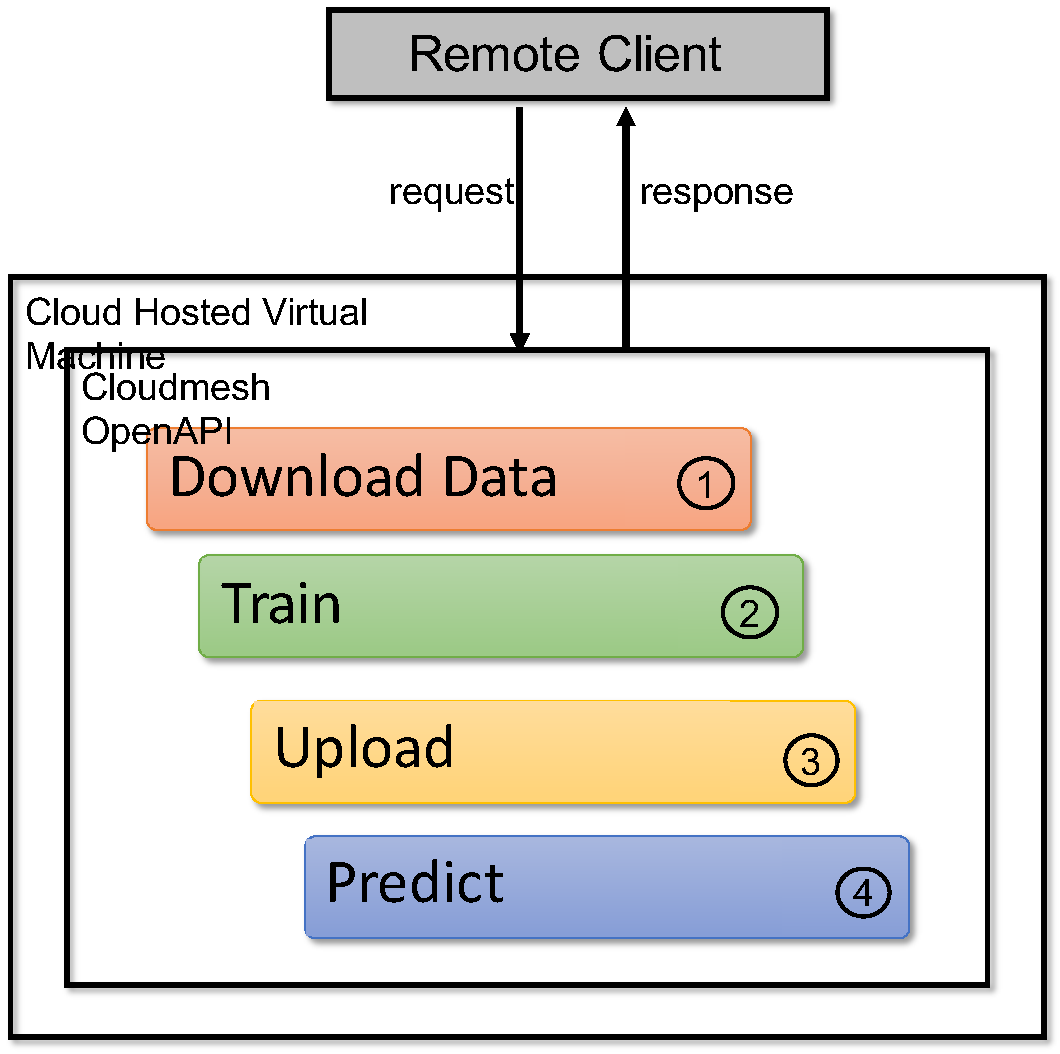
\includegraphics[width=0.7\columnwidth]{paper/images/architecture-openapi-1.pdf}

\caption{AI Service Workflow: A client running an AI service workflow, generated
and hosted by Cloudmesh OpenAPI, on a cloud provider virtual machine.
Requests for each function invocation are made using standard HTTP
request methods including function arguments.
}
\label{fig:1}
\end{figure}


\section{Multi-Cloud Hosted AI
Service}\label{multi-cloud-hosted-ai-service}

Cloudmesh with Cloudmesh OpenAPI provides a framework to deploy AI
services to multiple clouds. One use case for a multi-cloud deployment
is to benchmark cloud provider VM performance. A user can use these
tools to script the deployment of virtual machines with different
providers, virtual machine sizes, or operating systems. In Figure \ref{fig:2}, a
user has deployed an AI service hosted by Cloudmesh OpenAPI on three
separate cloud providers, AWS, Azure, and Google. The user makes
standard HTTP method requests to access the services simultaneously, and
gathers responses and benchmark statistics. With the Cloudmesh benchmark
utility, the user can measure the runtime of each AI service function
and collect key information such as virtual machine memory usage. This
information provides the user key insight for future hosting decisions.
We distinguish this example from Figure 1, where the AI service is
deployed on a single cloud provider.

\begin{figure}
\centering

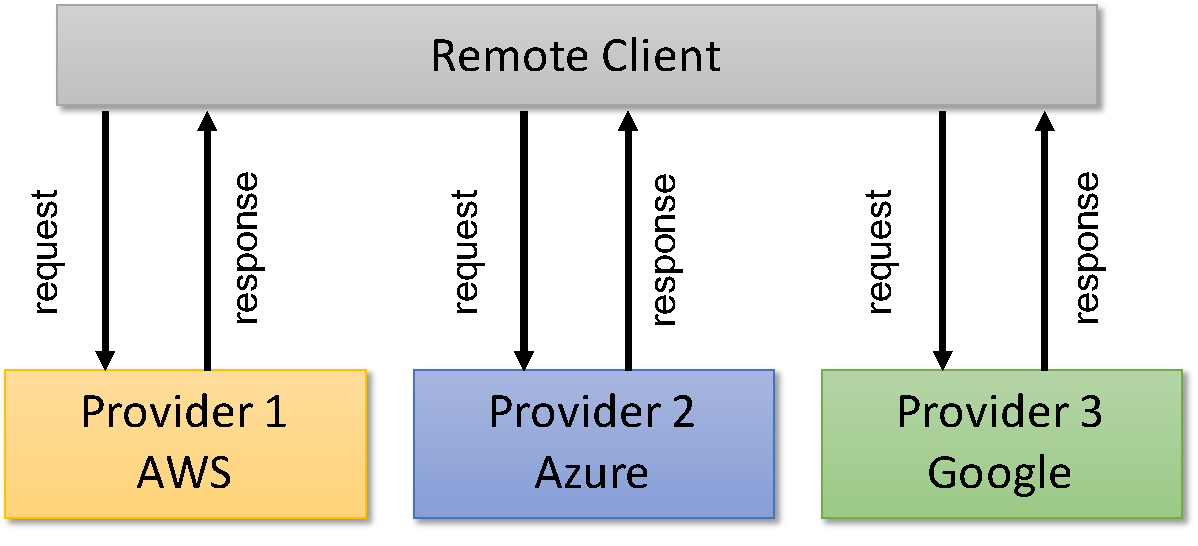
\includegraphics[width=\columnwidth]{paper/images/architecture-openapi-2.pdf}

\caption{Mult-Cloud AI Services: A client simultaneously accesses an AI service hosted
on three seperate cloud providers, AWS, Azure, and Google to benchmark
provider performance.}
\label{fig:2}
\end{figure}

\section{Benchmark}
\label{sec:benchmark}


We will develop benchmark tests that are pytest replications of Sklearn
artificial intelligent algorithms. These pytests will then be ran on
different cloud services to benchmark different statistics on how they
run and how the cloud performs. 

The team will obtain cloud service
accounts from AWS, Azure, Google, and OpenStack. To deploy the pytests,
the team will use Cloudmesh and its Openapi based REST services to
benchmark the performance on different cloud services. 

Benchmarks will
include components like data transfer time, model train time, model
prediction time, and more. The final project will include scripts and
code for others to use and replicate our tests. The team will also make
a report consisting of research and findings.

\subsection{Algorithms and Datasets}
\label{sec:algorithms-and-datasets}

This project uses a number of simple example algorithms and datasets. We
have chosen to use the examples included in Scikit Learn as they are
widely known and can be used by others to replicate our benchmarks
easily. Nevertheless, it will be possible to integrate easily other data
sources, as well as algorithms due to the generative nature of our base
code for creating REST services.

Within Skikit Learn we have chosen the following examples:

\begin{itemize}
\item
  \textbf{Pipelined ANOVA SVM}: An example code that shows a pipeline
  running successively a univariate feature selection with anova and
  then a SVM of the selected features \cite{www-skikit-learn-pipeline,}
\item
  \textbf{Eigenfaces SVM Facial Recognition}: A facial recognition
  example that first utilizes principle component analysis (PCA) to
  generate eigenfaces from the training image data, and then trains and
  tests a SVM model \cite{www-skikit-learn-faces}.

  This example uses the real world {\em Labeled Faces in the Wild} dataset
  consisting of labeled images of famous individuals gathered from the
  internet \cite{faces-data}.

\end{itemize}

\subsection{Cloud Providers}\label{cloud-providers}

Cloudmesh openapi works with virtual machine providers. It is necessary
to select similar virtual machines for benchmarking.

\hypertarget{aws}{%
\paragraph{AWS}\label{aws}}

\hypertarget{azure}{%
\paragraph{Azure}\label{azure}}

\hypertarget{google}{%
\paragraph{Google}\label{google}}

\hypertarget{openstack}{%
\paragraph{OpenStack}\label{openstack}}

\hypertarget{oracle}{%
\paragraph{Oracle}\label{oracle}}

\hypertarget{raspberry-pi-cluster}{%
\paragraph{Raspberry Pi Cluster}\label{raspberry-pi-cluster}}

\hypertarget{execution-on-raspbian}{%
\subparagraph{Execution on Raspbian}\label{execution-on-raspbian}}

\hypertarget{execution-on-a-kubernetes-cluster}{%
\subparagraph{Execution on a Kubernetes
Cluster}\label{execution-on-a-kubernetes-cluster}}

\begin{itemize}
\tightlist
\item
  \url{https://opensource.com/article/20/3/kubernetes-raspberry-pi-k3s}
\end{itemize}

\section{Result Comparision}\label{result-comparision}

In this section we will discuss the setup and execution of a benchmark
for three example AI services.

\subsection{VM Selection}\label{vm-selection}

When benchmarking cloud performance, it is important to identify and
control deployment parameters that can affect the performance results.
This enables one to analyze comparable services or identify
opportunities for service improvement for varying deployment features
such as machine size, location, network, or storage hardware. These
examples aimed to create similar machines across all three clouds and
measure service performance. See Table \ref{tab:1} for a summary of the parameters
controlled in these benchmark examples.

One key component is the virtual machine size, which determines the
number of vCPUs, the amount of memory, attached storage types, and
resource sharing policies. Resource sharing policies include shared
core machine varieties which providers offer at less expensive rates
and allow the virtual machines to burst over its base clock rate in
exchange for credits or the machines inherent bursting factor
\cite{amazon-instances,google-instances}. For this example, we chose
three similar machine sizes that had comparable vCPUs, comparable
underlying processors, memory, price, and were not a shared core
variety. We installed the same Ubuntu 20.04 operating system on all
three clouds.

Another factor that can affect performance, particularly in network
latency, is the zone and region selected. We deploy all benchmark
machines to zones on the east coast of the United States. This helps
control variations caused by network routing latency and provides more
insight into the inherent network performance of the individual cloud
services.

%\rowcolors{2}{gray!25}{white}

\begin{table*}
  
\caption{Selected VM parameters for benchmark measurement.
Clouds were tested at least twice, and were run sequentially between the
hours of approximately 1945 EST and 0330 EST starting with Google and
ending with Azure. * For the Eigenfaces SVM example, only 60 runs were
conducted on Azure due to a failed VM deployment from factors outside of
the benchnmark scripts control.}
\label{tab:1}

\begin{tabular}[]{@{}llll@{}}
\toprule
\begin{minipage}[b]{0.13\columnwidth}\raggedright
\strut
\end{minipage} & \begin{minipage}[b]{0.17\columnwidth}\raggedright
AWS\strut
\end{minipage} & \begin{minipage}[b]{0.47\columnwidth}\raggedright
Azure\strut
\end{minipage} & \begin{minipage}[b]{0.12\columnwidth}\raggedright
Google\strut
\end{minipage}\tabularnewline
\midrule
%\endhead
Size (flavor)
& 
m4.large
& 
Standard\_D2s\_v3 & 
n1-standard-2
\tabularnewline
vCPU & 2 & 2 & 2
\tabularnewline
Memory (GB) & 8 & 8 & 7.5
\tabularnewline
Image & ami-0dba2cb6798deb6d8
& \begin{minipage}[t]{0.80\columnwidth}\raggedright
Canonical:0001-com-ubuntu-server-focal:20\_04-lts:20.04.202006100\strut
\end{minipage} & 
ubuntu-2004-lts
\tabularnewline
OS & Ubuntu 20.04 LTS & Ubuntu 20.04 LTS & Ubuntu 20.04 LTS
\tabularnewline
Region & us-east-1 & eastus & us-east1
\tabularnewline
Zone &  N/A &  N/A & us-east1-b
\tabularnewline
Price (\$/hr)
&  0.1 & 0.096 & 0.0949995
\tabularnewline
Runs/Test
& \begin{minipage}[t]{0.17\columnwidth}\raggedright
90\strut
\end{minipage} & \begin{minipage}[t]{0.47\columnwidth}\raggedright
60*\strut
\end{minipage} & \begin{minipage}[t]{0.12\columnwidth}\raggedright
90\strut
\end{minipage}\tabularnewline
\bottomrule
\end{tabular}
\end{table*}

\subsection{Eigenfaces-SVM Example}\label{eigenfaces-svm-example}

We provide two example benchmarks for the Eigenfaces SVM example. The
first deploys and measures the AI service on a single cloud provider at
a time, and the second deploys a multi-cloud AI service, and then
measures the service across the clouds in parallel.

\subsubsection{Single Cloud Provider Service
Benchmarking}\label{single-cloud-provider-service-benchmarking}

The benchmark script for the Eigenfaces SVM example uses Cloudmesh to
create virtual machines and setup a Cloudmesh OpenAPI environment
sequentially across the three measured clouds including Amazon, Azure,
and Google. After the script sets up the environment, it runs a series
of pytests that generate and launch the Eigenfaces-SVM OpenAPI service,
and then conduct runtime measurements of various service functions.

The benchmark runs the pytest in two configurations. After the benchmark
script sets up a virtual machine environment, it runs the first pytest
locally on the OpenAPI server and measures five runtimes:

\begin{enumerate}
\def\labelenumi{\arabic{enumi}.}
\tightlist
\item
  Download and extraction of remote image data from
  ndownloader.figshare.com/files/5976015
\item
  The model training time when run as an OpenAPI service
\item
  The model training time when run as the Scikit-learn example without
  OpenAPI involvement
\item
  The time to upload an image from the server to itself
\item
  The time to predict and return the target label of the uploaded image
\end{enumerate}

The benchmark runs the second pytest iteration from the remote client it
is running on and interacts with the deployed OpenAPI service over the
internet. It tests two runtimes:

\begin{enumerate}
\def\labelenumi{\arabic{enumi}.}
\tightlist
\item
  The time to upload an image to the remote OpenAPI server
\item
  The time to run the predict function on the remote OpenAPI server, and
  return the target label of the uploaded image
\end{enumerate}

In Figure \ref{fig:3} we compare the download and extraction time of the labeled
faces in the wild dataset. This data set is approximately 233 MBs
compressed, which allows us to measure a non-trivial data transfer.
Lower transfer times imply the cloud has higher throughput from the data
server, less latency to the data server, or that it provides access to a
higher performing internal network. The standard deviation is displayed
to compare the variation in the download times.

\begin{figure}
\centering


\includegraphics[width=\columnwidth]{images/sample_graph_1.pdf}

\caption{Download Data Runtime:  Donwnload (233MB) and extraction
(\textasciitilde 275MB) of remote image data from
ndownloader.figshare.com/files/5976015.}
\label{fig:3}
\end{figure}

In Figure \ref{fig:4} we measure the training time of the Eigenfaces-SVM model
both as an OpenAPI service and as the basic Scikit-learn example. This
allows us to measure runtime overhead added by OpenAPI compared to the
source example. Here the two functions are identical except that the
OpenAPI train function makes an additional function call to store the
model to disk using joblib. This is necessary to share the model across
the train and predict functions. The standard deviation is displayed to
compare the variation in the training times.

\begin{figure}[htb]
\centering


\includegraphics[width=\columnwidth]{images/sample_graph_2.pdf}

\caption{Train Runtime: Compares the eigenfaces-svm model training time
running both as an OpenAPI service, and as the raw Scikit-learn example.
There are two bars per cloud provider. The bold bars are the training
time of the model when hosted as a Cloudmesh OpenAPI function. The
pastel bars are the training time of the Scikit-learn example code
without Cloudmesh OpenAPI involvement. The bars plot mean runtimes and
the error bar reflects the standard deviation of the runtimes.}
\label{fig:4}
\end{figure}

In Figure \ref{fig:upload} we measure the time to upload an image to the server both
from itself, and from a remote client. This allows us to compare the
function runtime as experienced by the server, and as experienced by a
remote client. The difference helps determine the network latency
between the benchmark client and the cloud service. The standard
deviation is displayed to compare the variation in the upload times.

\begin{figure}
\centering


\includegraphics[width=\columnwidth]{images/sample_graph_3.pdf}

\caption{Upload Runtime: Runtime of the upload function when run locally from
the OpenAPI server and from a remote client. There are two bars per
cloud provider. The bold bars are the runtime of the upload function as
experienced by the server, and the pastel as experienced by the remote
client. The bars plot mean runtimes and the error bar reflects the
standard deviation of the runtimes.}
\label{fig:upload}
\end{figure}


In Figure \ref{fig:predict} we measure the time to call the predict function on the
uploaded image. Again we run this once from the local server itself, and
a second time from a remote client to determine as experienced runtimes.
The standard deviation is displayed to compare the variation in the
predict times.

\begin{figure}
\centering


\includegraphics[width=\columnwidth]{images/sample_graph_4.pdf}

\caption{Predict Runtime Runtime of the predict function when run locally from
the OpenAPI server and from a remote client. There are two bars per
cloud provider. The bold bars are the runtime of the predict function as
experienced by the server, and the pastel as experienced by the remote
client. The bars plot mean runtimes and the error bar reflects the
standard deviation of the runtimes.}
\label{fig:predict}
\end{figure}

Table \ref{tab:2} presents a full listing of test results.

\TODO{why are there duplicated predit train? in table  \ref{tab:2}}

\begin{table}[htb]
  
\caption{Test results for the Eigenfaces SVM benchmark. Type
``local: denotes the test was run locally on the Cloudmesh Openapi
server, and remote denotes a remote host interacted with the server
using the python requets library.}
\label{tab:2}

\resizebox{1.0\columnwidth}{!}{
\begin{tabular}{lllrrrr}
\toprule
                   test &    type &   cloud &   mean &    min &    max &   std \\
\midrule
download data     &   local &     aws &  20.58 &  17.23 &  31.80 &  2.77 \\
download data     &   local &   azure &  20.81 &  13.56 &  42.70 &  6.94 \\
download data     &   local &  google &  18.00 &  17.06 &  19.38 &  0.48 \\
\midrule
predict           &   local &     aws &   0.03 &   0.02 &   0.05 &  0.00 \\
predict           &   local &   azure &   0.02 &   0.01 &   0.03 &  0.00 \\
predict           &   local &  google &   0.03 &   0.01 &   0.06 &  0.00 \\
\midrule
predict           &  remote &     aws &   0.40 &   0.26 &   0.80 &  0.18 \\
predict           &  remote &   azure &   0.36 &   0.24 &   0.60 &  0.13 \\
predict           &  remote &  google &   0.36 &   0.27 &   0.82 &  0.16 \\
\midrule
scikitlearn train &   local &     aws &  35.89 &  35.11 &  46.45 &  1.77 \\
scikitlearn train &   local &   azure &  40.13 &  34.95 &  43.96 &  3.29 \\
scikitlearn train &   local &  google &  42.13 &  41.77 &  42.49 &  0.13 \\
\midrule
train             &   local &     aws &  35.72 &  34.91 &  46.50 &  1.73 \\
train             &   local &   azure &  40.28 &  35.30 &  47.50 &  3.32 \\
train             &   local &  google &  42.04 &  41.52 &  45.93 &  0.71 \\
\midrule
upload            &   local &     aws &   0.01 &   0.01 &   0.01 &  0.00 \\
upload            &   local &   azure &   0.01 &   0.00 &   0.01 &  0.00 \\
upload            &   local &  google &   0.01 &   0.01 &   0.01 &  0.00 \\
\midrule
upload            &  remote &     aws &   0.43 &   0.16 &   1.13 &  0.21 \\
upload            &  remote &   azure &   0.32 &   0.15 &   0.50 &  0.15 \\
upload            &  remote &  google &   0.31 &   0.18 &   0.73 &  0.18 \\
\bottomrule
\end{tabular}
}

\bigskip

\caption{Test results for the Eigenfaces SVM benchmark deployed
  as a mutli-cloud service.}
\label{tab:3}

\resizebox{1.0\columnwidth}{!}{
\begin{tabular}{lllrrrr}
\toprule
test & type & cloud & mean & min & max & std \\
\midrule
download data & remote & aws    & 20.51 & 17.57 & 34.42 & 3.82 \\
download data & remote & azure  & 18.60 & 13.49 & 32.65 & 4.53 \\
download data & remote & google & 17.90 & 17.13 & 21.86 & 0.85 \\
\midrule
predict       & remote & aws	&  4.15 &  3.59 &  5.42 & 0.57 \\
predict       & remote & azure 	&  3.93 &  3.40 &  6.65 & 0.74 \\
predict       & remote & google &  4.13 &  3.74 &  6.37 & 0.60 \\
\midrule
train 	      & remote & aws 	& 35.61 & 35.24 & 39.53 & 0.73 \\
train 	      & remote & azure 	& 35.89 & 35.08 & 40.00 & 0.95 \\
train 	      & remote & google & 41.98 & 41.58 & 45.71 & 0.71 \\
\midrule
upload 	      & remote & aws 	& 10.08 &  4.89 & 16.52 & 4.38 \\
upload 	      & remote & azure 	&  8.46 &  4.72 & 13.92 & 4.05 \\
upload 	      & remote & google &  8.87 &  5.39 & 15.44 & 4.52 \\
\bottomrule
\end{tabular}
}


\end{table}

\subsubsection{Multi-Cloud Service Benchmarking}
\label{multi-cloud-service-benchmarking}

In this benchmark our script first acquires VMs, install Cloudmesh
OpenAPI, and launch the Eigenfaces SVM AI service on three separate
cloud providers. Because Cloudmesh has limited parallel computing
support, the script deploys the VMs in a serial manner. After the
services are running, we then run our tests in a parallel manner as
depicted in Figure 2. Testing in parallel provides faster benchmark
results, and better equalizes benchmark testing conditions. The
benchmark conducts requests to each cloud in parallel, so they should
experience similar network conditions. For example, in a serial testing
model, the remote data server may experience varying loads resulting in
different load times. Our parallel tests better equalize these
conditions by having each cloud download the data at the same time.

In Figure \ref{fig:7} we depict the combined runtime of our benchmark tests. This
allows us to compare the complete execution time of an AI service
workflow.

\begin{figure}
\centering
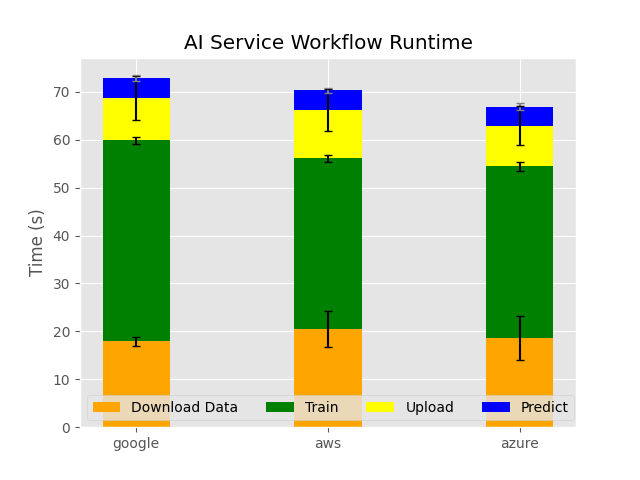
\includegraphics[width=\columnwidth]{images/ai_service_workflow_runtime.png}
\caption{AI Service Workflow Runtime: Mean runtime of the Eigenfaces SVM workflow deployed
as a multi-cloud service. We compute the means from 30 runs of a
workflow that included 1 download data invocation, 1 train invocation,
30 upload invocations, and 30 predict invocations. We run the workflows
in parallel on the separate clouds using a multiprocessing on an 8-core
machine.}
\label{fig:7}
\end{figure}

In Table \ref{tab:3} we provide complete test results.



\subsection{Pipelined Anova SVM Example}
\label{pipelined-anova-svm-example}

\subsection{Caleb Example}\label{caleb-example}

\section{Limitations}\label{limitations}

Azure has updated their libraries and discontinued the version 4.0 Azure
libraries. We updated Cloudmesh to use the new library, but not all
features, such as virtual machine delete, are implemented or verified.

\section{Conclusion}
\label{sec:conclusion}

\TODO{TBD}


\section*{Acknowledgements}\label{acknowledgements}

We like to thank
\href{https://github.com/cybertraining-dsc/fa20-523-325/}{Vishwanadham
Mandala} to participate in helping write an earlier version of this
document.

\bibliographystyle{ACM-Reference-Format}
\bibliography{references}

\clearpage

\appendix

\section{Appendix}

\subsection{Setup}\label{appendix-a.---setup}

\subsubsection{Deployment}\label{a.1.-deployment}

The project is easy to replicate with our detailed instructions. First
you must install Cloudmesh OpenAPI whihch can be done by the following
steps:


\begin{verbatim}
python -m venv ~/ENV3
source ~/ENV3/bin/activate 
mkdir cm
cd cm
pip install cloudmesh-installer
cloudmesh-installer get openapi 
cms help
cms gui quick
# fill out mongo variables
# make sure autinstall is True
cms config set cloudmesh.data.mongo.MONGO_AUTOINSTALL=True
cms admin mongo install --force
# Restart a new terminal to make sure mongod 
# is in your path
cms init
\end{verbatim}
 

As a first example we like to test if the deployment works by using a
number of simple commands we execute in a terminal.

\begin{verbatim}
cd ~/cm/cloudmesh-openapi

cms openapi generate get_processor_name \
    --filename=./tests/server-cpu/cpu.py

cms openapi server start ./tests/server-cpu/cpu.yaml

curl -X GET "http://localhost:8080/cloudmesh/get_processor_name" \
     -H "accept: text/plain"
cms openapi server list

cms openapi server stop cpu
\end{verbatim}

The output will be a string containing your computer.

\TODO{how does the string look like}


As we often also need the information as a REST service, we provide in
our next example a jsonified object specification.

\begin{verbatim}
from flask import jsonify

def add(x: float, y: float) -> str:
    """
    adding float and float.
    :param x: x value
    :type x: float
    :param y: y value
    :type y: float
    :return: result
    :return type: float
    """
    result = {"result": x + y}

    return jsonify(result)
\end{verbatim}

The result will include a json string returned by the service.

\begin{verbatim}
cms openapi generate add --filename=./tests/add-json/add.py
cms openapi server start ./tests/add-json/add.yaml 
curl -X GET "http://localhost:8080/cloudmesh/add?x=1&y=2" \
     -H "accept: text/plain"
# This command returns
> {"result":3.0}
cms openapi server stop add
\end{verbatim}

These examples are used to demonstrate the ease of use as well as the
functionality for those that want to replicate our work.


\subsection{Pipiline ANOVA SVM}\label{a.2.-pipiline-anova-svm}

This example demonstrates how to deploy a simple machine learning
example onto a server using cloudmesh-openapi. The specific
implementation details that this example is based on can be found
\href{https://scikit-learn.org/stable/auto_examples/feature_selection/plot_feature_selection_pipeline.html}{here.}

The model being implemented is, in essence, an SVM with extra features
to improve the model. An SVM (support vector machine) is a supervised
learning model with associated learning algorithms used for
classification and regression analysis. This model has become one of the
most robust prediction methods widely used in problems conerning
classification and the like.

The Pipeline and ANOVA aspects are extensions to the SVM to improve the
overall model. The purpose of the pipeline is to assemble several steps
that can be cross-validated together while setting different parameters.
ANOVA on the other hand is an acronym for Analysis of Variance. It is an
omnibus test, meaning it tests for a difference overall between all
groups. In the context of an SVM, this information is useful as an SVM
mainly classifies data into separate groups.

We can now proceed as follows:

\begin{verbatim}
$ pwd
~/cm/cloudmesh-openapi

$ cms openapi generate PipelineAnovaSVM \
      --filename=./tests/Scikitlearn-experimental/sklearn_svm.py \
      --import_class --enable_upload

$ cms openapi server start ./tests/Scikitlearn-experimental/sklearn_svm.yaml
\end{verbatim}

After running these commands, we opened a web user interface. In the
user interface, we uploaded the file iris data located in
\verb|~/cm/cloudmesh-openapi/tests/|
Scikitlearn-experimental/iris.data

We then trained the model on this data set by inserting the name of the
file we uploaded \verb|iris.data|. Next, we tested the model by
clicking on make\_prediction and giving it the name of the file
iris.data and the parameters \verb|5.1|, \verb|3.5|, \verb|1.4|,
\verb|0.2|

The response we received was
\verb|Classification: ['Iris-setosa']|

Lastly, we close the server:

\begin{verbatim}
$ cms openapi server stop sklearn_svm
\end{verbatim}

This process can easily be replicated when we create more service
examples that we derive from existing sklearn examples. We benchmark
these tests while wrapping them into pytests and run them on various
cloud services.

\subsection{Eigenfaces SVM Facial
Recognition}\label{a.3.-eigenfaces-svm-facial-recognition}

Next we demonstrate how to run the Eigenfaces SVM example locally, and
then how to run its associated benchmark script.

\begin{verbatim}
$ pwd
~/cm/cloudmesh-openapi

$ git checkout benchmark # todo required until merged into main

$ cms openapi generate EigenfacesSVM \
      --filename=./tests/generator-eigenfaces-svm/eigenfaces-svm-full.py \
      --import_class --enable_upload

$ cms openapi server start \
      ./tests/generator-eigenfaces-svm/eigenfaces-svm-full.yaml
\end{verbatim}

After running these commands, we opened a web user interface at
\url{http://localhost:8080/cloudmesh/ui}. In the user interface we run
the download\_data function with the default arguments. This downloads
and extracts the labeled faces in the wild data set to the
\verb|~/scikit_learn_data/lfw_home directory|.

Next, we run the train function to train the model. The train function
performs a 50/50 train/test split on the input data, and returns
performance statistics of the trained model.

Next, we use the upload function to upload an example image using
\verb|~./tests/generator-eigenfaces-svm/example\_image.jpg|
as the function argument. This puts the example image in the
\verb|~/.cloudmesh/upload-file/| directory.

Finally, we run the predict function with the uploaded file path as an
argument,
\verb|~/.cloudmesh/upload-file/example\_image.jpg|,
and receive the classification as a response
\verb|['George W. Bush']|

Last, we close the server:

\begin{verbatim}
$ cms openapi server stop EigenfacesSVM
\end{verbatim}

Next, we benchmark these tests while wrapping them into pytests and run
them on various cloud services.

\textbf{Before continuing you must have successfully registered AWS,
Azure, and Google clouds in your yaml file and be able to boot virtual
machines on Google, AWS, and Azure. This example currently should work
on Linux and macOS}

First, we must change to a git branch that includes Azure provider
fixes, and setup our \verb|~./cloudmesh/cloudmesh.yaml| file to
replicate the parameters set for the benchmark results above. This can
be done with the commands listed in Figure \ref{fig:config}.

\TODO{NEVER USE THE WORD ABOVE to refer to previous, next or numbered items}

\begin{figure*}[htb]

\begin{verbatim}
$ cd ~/cm/cloudmesh-azure 
$ git checkout benchmark # required until changes merged to main

$ cd ~/cm/cloudmesh-openapi

$ cp ~/.cloudmesh/cloudmesh.yaml ~/.cloudmesh/cloudmesh.bak.1 # to revert reverse the cp

$ cms config set cloudmesh.cloud.azure.default.image="Canonical:0001-com-ubuntu-server-focal:20_04-lts:20.04.202006100"
$ cms config set cloudmesh.cloud.azure.default.size="Standard_D2s_v3"
$ cms config set cloudmesh.cloud.azure.credentials.AZURE_REGION="eastus"

$ cms config set cloudmesh.cloud.aws.default.image="ami-0dba2cb6798deb6d8"
$ cms config set cloudmesh.cloud.aws.default.size="m4.large"
$ cms config set cloudmesh.cloud.aws.default.username="ubuntu"
$ cms config set cloudmesh.cloud.aws.credentials.region="us-east-1"

$ cms config set cloudmesh.cloud.google.default.image="ubuntu-2004-lts"
$ cms config set cloudmesh.cloud.google.default.image_project="ubuntu-os-cloud"
$ cms config set cloudmesh.cloud.google.default.zone="us-east1-b"
$ cms config set cloudmesh.cloud.google.default.region="us-east1"
$ cms config set cloudmesh.cloud.google.default.flavor="n1-standard-2"
\end{verbatim}

  \caption{Configuration}
  \label{fig:config}
  \end{figure*}

Next, we will modify the default security group to open the flask server
port 8080 for OpenAPI service testing.

\begin{verbatim}
$ cms sec rule add openapi 8080 8080 tcp 0.0.0.0/0
$ cms sec group add default openapi for_openapi_demo
# the above two command should allow aws and azure to work
# sec group load is broken for google and it does not 
# use the default sec group, so you have to manually 
# add the openapi rule to google cloud for now
# console.cloud.google.com > VPC network > firewall > create firewall rule
# name: openapi, targets:  all instances in network, 
#       Source IP ranges: 0.0.0.0 /0, 
#       specified protocols and ports: tcp 8080 > create
\end{verbatim}

Next, we will run the benchmarking script,

\verb|./tests/generator-eigenfaces-svm/benchmark-eigenfaces.py.|

This script utilizes the Cloudmesh shell and the Bash script,

\verb|./tests/generator-eigenfaces-svm/eigenfaces-svm-full-script|,

to sequentially deploy a VM on each of the clouds, install
Cloudmesh-openapi and the example dependencies, and then us the
pytest, \\
\verb|./tests/test\_030\_generator\_eigenfaces\_svm.py|, twice to
benchmark the EigenfacesSVM service functions both locally from the
server, and from the remote client running the benchmark
script. Finally, it prints and plots performance statistics.

\begin{verbatim}
$ ./tests/generator/eigenfaces-svm/benchmark-eigenfaces.py run
\end{verbatim}

If the command line argument \verb|run| is passed to the script, then
it will start up the virtual machines on each cloud. Output and
benchmark results from each of the virtual machines will be store in the
\verb|~/.cloudmesh/eigenfaces-svm/vm\_script_output/| directory.
The benchmark results are scraped from the script outputs and stored in
the \verb|~/.cloudmesh/eigenfaces-svm/benchmark_output|
directory. If the \verb|run| argument is \textbf{not} provided, it
will only print statistics from script output already stored in the
vm\_script\_output directory.

Statistics will be printed to the command line, and graphs will be
displayed using plt.show() function calls as well as saved to the \\
\verb|./tests/generator-eigenfaces-svm/ directory|.

Next, we will run the multi-cloud benchmarking script,

\verb|.tests/generator-eigenfaces-svm/bencmark-eigenfaces-multi-cloud.py|.

This script uses the Cloudmesh shell and the Bash script,

\verb|.tests/generator-eigenfaces-svm/eigenfaces-svm-full-multi-script|,

to sequentially deploy a VM on each of the clouds, install
Cloudmesh-OpenAPI and the example dependencies, and start the AI
service. Next, it conducts HTTP requests in parallel to interact with
the services to measure the runtime for data download, training,
uploading, and prediction.

\begin{verbatim}
$ ./tests/generator/eigenfaces-svm/benchmark-eigenfaces-multi-cloud.py run
\end{verbatim}

As above the command line argument run is used to conduct actual tests,
and the absence of that argument simply computes statistics on existing
output from the \\
\verb|~/.cloudmesh/eigenfaces-svm/vm_script_output_multi/|
directory.

Statistics will be printed to the command line, and graphs will be
displayed using plt.show() function calls as well as saved to the
\verb|./tests/generator-eigenfaces-svm/ directory|.

\subsection{Using unit tests for
Benchmarking}\label{a.4.-using-unit-tests-for-benchmarking}

\TODO{This section will be expanded upon}

\begin{itemize}
\item
  Describe why we can unit tests
\item
  Describe how we access multiple clouds

\begin{verbatim}
cms set cloud=aws
# run test
cms set cloud=azure
# run test
\end{verbatim}
\item
  Describe the Benchmark class from cloudmesh in one sentence and how we
  use it

\subsection{APPENDIX C. - Cloudmesh
Links}\label{appendix-c.---cloudmesh-links}

We added this section so the Reader can easily find some cloudmesh
related information Documentation for Cloudmesh can be found at \cite{cloudmesh-manual}:

Code for cloud mesh can be found at \cite{cloudmesh-github}.

Examples in this paper came from the cloudmesh openapi manual which is
located here \cite{cloudmesh-openapi}.

Information about cloudmesh can be found here \cite{cloudmesh-manual},
whic includes various cloudmesh installations documentation for
different OSes.

\subsection{APPENDIX D. - Plan}\label{appendix-d.---plan}

\cite{www-skikit-learn-faces}.

\section{YAML}

\TODO{TBD}


\begin{figure}[!h]
%\begin{Verbatim}[numbers=left,xleftmargin=5mm]
\bigskip
\begin{lstlisting}[language=Python,
                   basicstyle=\ttfamily\footnotesize,
                   numbers=left,                   
                   numbersep=5pt,
                   xleftmargin=5mm]
openapi: 3.0.0
info:
  title: Calculator
  description: "A simple calculator that allows you to do basic math operations"
  version: "1.0"
servers:
  - url: http://localhost:8080/cloudmesh
    description: "A simple calculator that allows you to do basic math operations"
paths:
  /Calculator/dividefloat:
     get:
      summary: "Divide int by float."
      description: "None (Optional extended description in CommonMark or HTML)"
      operationId: calculator.Calculator.dividefloat
      parameters:
        - in: query
          name: x
          description: "the value of input #1"
          schema:
            type: integer
        - in: query
          name: y
          description: "the value of input #2"
          schema:
            type: number
      responses:
        '200':
          description: "OK"
          content:
            text/plain:
              schema:
                type: number

  /Calculator/multiplyint:
     get:
      summary: "Multiply int by int."
      description: "None (Optional extended description in CommonMark or HTML)"
      operationId: calculator.Calculator.multiplyint
      parameters:
        - in: query
          name: x
          description: "the value of input #1"
          schema:
            type: integer
        - in: query
          name: y
          description: "the value of input #2"
          schema:
            type: integer
      responses:
        '200':
          description: "OK"
          content:
            text/plain:
              schema:
                type: integer
                

\end{lstlisting}

\caption{YAML file generated from the python function}
\label{fig:class-yaml}

\end{figure}


\TODO{TBD}

\clearpage